\documentclass[12pt,a4paper]{article}
\usepackage[utf8]{inputenc}
\usepackage[english]{babel}
\usepackage{amsmath}
\usepackage{amsfonts}
\usepackage{amssymb}
\usepackage[left=2.00cm, right=2.00cm]{geometry}
\usepackage{graphicx}
\usepackage{xcolor}
\usepackage{natbib}
\usepackage{comment}
%\usepackage[style=authoryear-icomp,sorting=anyt]{biblatex}

%\addbibresource{Biblio_deepbios.bib}
%\graphicspath{C:\Users\Rodrigo\Desktop\Papers_ON GOING\TREE_Modelling}

\begin{document}
\title{Evolving computational sustainability in rapidly changing exploited ecosystems}

\maketitle
\noindent \author{Rodrigo Riera$^{1,2,*}$, Ali Vadathi$^{3}$, Gian Marco Palamara${^3}$, David Alonso${^4}$, Joaqu\´in Hortal${^5}$, and Carlos J. Meli\´an${^6}$}
            \\
            %TO ADD VICTOR EGUILUZ --- FRANCISCO BALDO -- 
            
            %Potential coauthors: 
            %JON NORBERG -- PAULO GUIMARAES -- PENGJUAN ZU
            %In case we use RLS global database, it is mandatory to include Graham Edgar and Rick Stuart-Smith
            \vspace{0.25 in}
            
  \noindent  $^{1}$IU-ECOAQUA, Departamento Biolog\'ia, Universidad de Las Palmas de Gran Canaria, Canary Islands, Spain\\
  $^{2}$Departamento de Ecolog\'ia, Facultad de Ciencias, Universidad Cat\'olica de la Sant\'isima Concepci\'on, Concepci\'on, Chile\\
  $^{3}$, Switzerland\\
  $^{3}$Department of System Analysis, Integrated Assessment and Modelling, EAWAG Center for Ecology, Evolution and Biogeochemistry, Switzerland\\
  $^{4}$Theoretical and Computational Ecology, Center for Advanced Studies of Blanes, Girona, Spain\\
  $^{5}$Departamento de Biogeograf\'ia y Cambio Global, MNCN, Madrid, Spain\\
  $^{6}$Department of Fish Ecology and Evolution, EAWAG Center for Ecology, Evolution and Biogeochemistry, Switzerland\\
\vspace{0.25 in}

  $^{*}$corresponding author: rodrigo.riera@ulpgc.es

\newpage
\section{Abstract}
Biodiversity research is being rapidly transformed by novel analytical methods and data integration. Recent studies have shown processes and patterns in changing ecosystems are driven by fine-grained biological-human interactions, but also by coarse-grained Earth and environmental dynamics. Yet, deciphering the strength of the coupling connecting Environmental, Social, Earth and Biodiversity science is at a very incipient stage. Here we identify three main challenges to integrate Environmental, Social, Earth and Biodiversity science into a unified computational sustainability framework: (i) We expand toy models with explainable Bayesian network models; (ii) We explore gradients of complexity in the modeling framework to decipher the mechanisms for large and complex ecosystems, and (iii) We validate our approach with a case study focusing on the sustainability of the oceans in federated networks, where many heterogeneous groups of species, humans, and technologies coexist exploiting resources in complex ecosystems. Lastly, we discuss our approach in the context of open-source software solutions for the development of science-enabled technologies aiming to connect knowledge-inspired societies to global sustainability challenges.


\begin{comment}
The merging of pattern- and process-based methods and the building
of theory to merge knowledge and predictive power is not taken
place. Theories play a pivotal role in providing explanations to
what, at first, might seem to be a series of disconnected, even
paradoxical, patterns. We provide here a framework connecting
synthesis between pattern- and process-driven research. Our approach
integrates deep learning networks with process-based methods, i.e. deep
process-based learning network to infer patterns and processes
underlying large and integrated databases. We show a case study
using a deep process-based learning network to explore the strength of
coupling between layers and the dimensionality in Biodiversity and
Environmental databases. We validate our approach with a case study focusing on the sustainability of the oceans in federated networks, where many heterogeneous groups of species, humans, and technologies coexist exploiting resources in complex ecosystems. Merging process-based approaches and
data-driven deep learning networks might play a critical role in
deciphering the strength of the coupling between Earth and
biodiversity systems in rapidly changing landscapes. Lastly, this project not ly sets out to deliver novel computational sustainability approaches but also provides fully reproducible open-source software solutions of a science-enabled technology to connect knowledge-inspired societies to global sustainability challenges.
\end{comment}

\newpage

\section{Introduction}
Human footprint is pervasive worldwide, with no such a thing as untouched wilderness \citep{marconcini2020outlining, mcdowell2020pervasive}. Biodiversity research is a top priority to ensure ecosystem conservation and halting habitat loss and fragmentation \citep{brum2017global}. Unraveling the linkages among physico-chemical processes, environmental drivers, internal regulatory processes at the population, community, and ecosystem levels; and the role of human intervention is essential for effective management and sustainability \citep{hobbs2011intervention}. Recent approaches have shown that these interactions can result in complex dynamical behavior including sudden shifts in ecosystem states and extinction patterns of populations and communities \citep{newman2019scaling}. Biodiversity science has expanded in a wide range of sub-disciplines throughout the last decades \citep{loreau2010challenges}, yet, integrating database to decipher the sustainability properties of exploited ecosystems is at a very incipient stage. Exploited ecosystems need to be addressed from a broad-scale and synthesis perspective, because of the complex scientific problems concerning the description and prediction of biodiversity patterns and processes using data from genes, individuals, communities, and ecosystems across temporal and spatial scales \citep{chase2018embracing}, as well as, their implications on current and future societal challenges such as, climate change, human health and poverty \citep{cardinale2012biodiversity, turner2012global}.

Connecting exploited to biodiversity maintenance is calling for technologies to discover novel ways of sustainable exploitation. Novel technologies for data integration from different fields, i.e. environmental, social, biodiversity and Earth science data, can uncover new patterns, causal relationships and new paths to reach sustainable exploitation while maintaining biodiversity. This is of paramount importance since the patterns observed in ecosystem's collapse are usually driven by the interactions among different agents, sectors, and spatio-temporal scales.
Major technological advances in computing power, remote sensing, and omics, i.e. genomics, transcriptomics, proteomics, metabolomics, among others, have provided new tools to improve understanding of biodiversity patterns \citep{craven2019evolution}. These advances within the framework of knowledge-based societies place great expectations on data-driven intelligent machines to face global sustainability challenges. In this regard, database integration to facilitate the discovery of sustainable paths in resource exploitation, the major feature of computational sustainability, is a major issue revolving around data-driven intelligent machines and knowledge-based societies \citep{Gomesetal2019}. 

However, there are still considerable limitations regarding the integration of data and modelling approaches, especially those concerning the (i) connections between oversimplified toy models and more realistic counterparts, and (ii) computational constraints when developing complex and realistic models. There have recently been fast improvements in methods delivering explainable and complex models integrating heterogeneous data, and also, these models challenge the limits to computational speed to deliver robust conclusions \citep{rodrigues2014integrative}. Moreover, there is still way to go through interdisciplinary fields that promote synergies among societal, economic, and environmental resources within the framework of sustainability. The main core sustainability themes remain dispersed and integrated only superficially: (i) Biodiversity and Conservation; (ii) Balancing environmental and socio-economic needs; and (iii) Energy and renewable resources. Only recently, new tools for data integration and analysis, can facilitate the integration required to gain understanding between exploited and sustainable ecosystems for species-rich and human-dominated ecosystems.

Here we aim to explore model's complexity gradients using Bayesian networks to uncover relations among the data, causality graphs and novel paths to broaden computational sustainability concepts (see Table and methods). Our integration has the potential to integrate process- and pattern-based models from toy to more complex ones to optimize a wide range of resources, i.e. diverse prey communities, environmental factors, fishing and the technologies used to exploit resources and the economic or societal impacts. Scaling up from micro-ecological processes requires the use of data driven evidence, and it is essential that data from implementation monitoring are linked to decision making through data integration and model's complexity gradients robustly explored. 

Therefore, integrating data, causality and novel paths to connect exploitation and sustainability criteria in complex ecosystems can assist both policy makers and researchers to determine the most useful type of research at different stages of scaling up processes. This process is of paramount importance to avoid failure of initiatives to influence the society, and the "know-do gap" - the gap between what is known in research and what gets implemented \citep{catford2009advancing}. 

The migration from toy to deep learning models will expand the reach of an intervention to new settings or target groups and is accompanied by systematic strategy to achieve this objective \citep{milat2014increasing}. Yet, scarce studies deal with frameworks, approaches and methods for effective scale-up interventions \citep{wigboldus2013towards, yamey2012barriers}. The integration of deep learning networks with process-based methods providing evidence-to-practice frameworks are pivotal for policy makers, practitioners and stakeholders to scale up global interventions. Computational sustainability is an interdisciplinary discipline that needs to be built from a federated network, potentially more powerful than centralized ones. Many computational sustainability problems require making decisions through time, solving these problems involve maximizing expected reward by finding the most suitable that can generate future hypotheses without considering the simulator to run. Another approach consists of the recently developed "stochastic computers" \citep{borders2019integer}, energetically more efficient than conventional ones, and perform faster and more complex calculations. Yet, complex and integrative computational analysis are laborious and extremely time-consuming \citep{rodrigues2014integrative}, especially those related to big data involved in deep learning approaches. Several alternatives have been recently developed such as, the development of off-policy evaluation using Model Free Monte Carlo (MFMC) method \citep{fonteneau2010model}. 

%The modeling framework in federated networks aiming to (i) connect toy to explainable deep learning models and (ii) obtain robust inference even for large and complex models 
Diversification of biological systems offers an unexplored avenue for inspiration of new computational approaches. However, diversifying ecosystems are not used for sustainability discovery yet, despite the rapid changes of traits and interactions observed in overexploited, experimental and theoretical systems \citep{Hairston2005, Walsh2006, Fussmann2007, Trugman8532}. Biological systems are characterized by feedbacks between the ecology and evolution of interacting traits, the eco-evolutionary feedbacks, to produce novel traits with new functionalities \citep{Govaertetal2019}. This results in new computational properties, like new cooperation and competition strategies and information processing capabilities. Diversification usually occurs in heterogeneous ecosystems with limited resources where many distinct groups need to develop specialized traits and strategies to obtain resources. The outcome is the formation of consortia and more broadly federated networks composed of phylogenetically and ecologically distinct groups. Conventional Artificial Intelligence (AI) is rapidly moving towards explainable and discovery pattern inference \citep{Iten2020a} but often avoids evolutionary diversification for exploring new computing capabilities \citep{Real2020}. The same situation occurs for artificial neural networks that also make limited use of novel computing capabilities as a consequence of new interactions and traits \citep{Schmidhuber:2015}.

%This paragraph has been largely amended to improve (hope so!) the main idea and aims of the paper. The last paragraphs are taken from the abstract, and need to be polished accordingly.
\textbf{The goal of this project is to implement eco-evolutionary diversification-inspired solutions to perform computational sustainability discovery based on rapidly diversifying traits and interactions}. The exploitation of emerging interactions, strategies and traits will allow us to create novel discovery solutions for natural ecosystems facing sustainability challenges like overexploitation of the oceans, where harvesting renewable resources are beyond the diminishing returns for many species and ecosystem resources \citep{Paulyetal1998, Mastrangelo2019}. Why should we go deeper into diversifying networks for computational sustainability? With connections and traits represented in a spatially distributed network, as found in natural ecosystems, diversification is an avenue to harvest renewable resources because most innovations in ecosystems are connected to new sensing and information processing cues to detect and exploit resources. This allows considering not only evolutionary processes changing traits and agents (i.e., plasticity and other sources of variation), but the formation of new entities to quantify new scenarios for sustainability that substantially deviate from evolutionary computation considering only changes and not diversification processes. This also allows representing real-time solutions for ever-changing renewable resources, which is a key problem in many digital and natural systems. We here show a case study using a deep process-based learning network to explore the strength of
coupling between layers and the dimensionality in Biodiversity and Environmental databases. We test this approach with a case study focusing on the ocean sustainability in federated networks, where species, humans, and technologies coexist exploiting resources in complex and rapidly changing seascapes. To show the capabilities of the approach, we will address full reproducibility, automation, visualization, and reporting (Figure 1). The integration of data, causality and diversity may provide a new technology to improve ecosystem sustainability relevant to community-rich digital and natural ecosystems.


%\begin{tabular}%[leftmargin=2cm]
\begin{enumerate}%[\hspace{-0.0 in}(G1)]
%\setlength\itemsep{-0.3em}
   % \vspace{-0.15 in}
    \item To extend existing theories of eco-evolutionary diversification and AI-inspired solutions to decipher the factors driving sustainability discovery in federated networks. This will allow us to identify novel solutions for ecosystem sustainability.
% \vspace{-0.15 in}
    \item To investigate how spatio-temporal evolutionary diversification and AI-inspired networks mimic the empirical patterns of natural and socio-technological ecosystems when heterogeneous human groups, technologies, and species coexist.
% \vspace{-0.15 in}    
    \item To develop fast, reproducible and automated eco-evolutionary diversification-inspired sustainability discovery prototypes for real-time information processing tasks.
% \vspace{-0.15 in}    
    \item To obtain principles of sustainability discovery for prediction in federated networks when diversification in interactions and traits occurs in a large and heterogeneous set of species, technologies and human groups. 
\end{enumerate}

How can we develop robust and testable ecological theory taking into
account large and complex integrated datasets? First, biodiversity
data is typically scarce and biased (\citep{hortal2015seven}). Although an increasing number of ecological
datasets are available, most, if not all, of them are of uneven
coverage and quality (see Table 1). Second, many patterns have emerged
with conflicting explanations usually depending on the spatial and
temporal scales of the observations (see Table 2). Lastly, progress in
ecology relies on unifying different theories in order to explain as
many natural patterns with as fewer principles as possible. This
implies confronting models to obtain more robust theories. Also,
merging methods from distinct disciplines can increase our predictive 
understanding power to develop and test new theory (\citep{reichstein2019deep}). A series of approaches,
e.g. computational ecology, statistical physics, matrix theory, among
others, will be pivotal to fully integrate this marriage between empirical data and theory, particularly through guiding the attention of researchers onto integrating datasets to inference accounting for several biological levels and spatio-temporal scales \citep{melian2018deciphering}, \citep{poisot2019data}.

Conventionally, machine and deep learning, and research on
biodiversity have been considered as distinct fields. Recent
approaches in ecology and evolution have introduced deep learning
methods for labelled data, from which selection modes and demographic
history can be jointly inferred, among other things \citep{sheehan2016deep}. The fussion
of modern data analysis and theory in biodiversity research would shed
light on process-based scenarios of biodiversity decline. Yet, most approaches applying deep learning methods in biodiversity have mostly focused at one level of biological organization, e.g. genes, species
or communities, without considering the interaction among them. And
also, these studies are single-focused and limited to taxonomic
diversity, with no consideration of other emerging diversity
dimensions. Here, functional (trait-based) and phylogenetic
(phylogeny-based) approaches to community ecology have demonstrated to unravel the relevance of mechanisms driving species assembly and ecosystem functioning \citep{weiss2019unifying}. Biological systems are composed by many layers (Figure 1), and they can contain interdependent hierarchies and feedbacks with interacting learning
entities within and between the layers. The number of layers needed for predicting and understanding biological patterns still remains overlooked. This is specifically complex in the Anthropocene epoch, with the widespread role of human-driven disturbances. Deep process-based models need accounting for several layers and interactions within and between the layers \citep{fontaine2011ecological}, \citep{melian2018deciphering},
\citep{reichstein2019deep}). Data science and biological systems share
pivotal properties, but their full potential has not been sufficiently
explored \citep{schmidhuber2015deep}. Therefore, exploring deep
learning networks topologies accounting for feedbacks within and
between layers is a first step towards understanding biodiversity
dynamics using deep process-based learning networks.

\\
Make better flow between computational sustainability and data, causal, and discovery knowledge graphs -- make clear the case study
\\

\section{Methods: Integrating data, causal and discovery knowledge graphs}

\subsection{Emulating simulations in sustainable ecosystems}

Sustainable ecosystems are complex ones that incorporate several parameters and heterogeneity across levels. Deciding which level of complexity best capture real ecosystems for understanding sustainability is a major challenge today. Modeling such systems requires tools such as agent-based models integrating data from many fields. ABMs can show emergent properties and many of the features of a system that are often absent in analytical models. A draw back of ABMs is that they are computationally expensive. Therefore, methods making a continuum from analytical models to ABMs are required to quantitatively evaluate pros and cons of both approaches. Analyzing ABMs needs exploring a large parameter space, which is usually not feasible. A work around for this limitation is building emulators, which are mathematical formulations (machine learning models) that can estimate the complex behavior of a simulation given different inputs. We can use either traditional machine learning algorithms or deep learning for this endeavour. Traditional ML algorithms have a limited predictive power and may not be able to predict complex high dimensional data. Deep learning is often the choice when there are large number of training samples. But such large number of samples are not easy to produce when single simulation runs themselves take long. A solution to this problem is to find an optimal deep learning architecture. This has been shown to be able to replace complex simulations with very few input data (\cite{Kasim2020}). There are different optimization methods for finding the best architecture (\cite{Elsken2018}). Here, we explore architectures with different degrees of complexity aiming to unify analytical to ABMs scenarios to understand the paths to sustainable ecosystems. 

Emulators are required when our available data is incomplete. It can happen in two cases. First, when we are producing simulated data and those simulations are too time consuming to explore all parameter combinations. Second, when we have experimental data that are hard to gather and do not cover all possible parameter combinations. Emulators can predict how the system (computational or real) would behave with new parameter values. These predictions would then be valuable to create knowledge graphs to answer sustainability questions (i.e., finding discovery paths that improve sustainability in the exploitation of the ecosystem).

\subsection{Probabilistic graphical models}

Probability graphical models (PGMs), a subset of which are Bayesian Networks (BNs) are a powerful tool for mixing available data (from computer simulations, experiments, and expert knowledge) to gain a comprehensive understanding of a complex ecosystem. An advantage of BNs is that they provide probabilistic answers taking into account the uncertainties in data collection and outputs. In BNs are directed acyclic graphs (DAG) that show causation between different parameters. They allow us to explore the effect of changing one parameter on parameters that are connected to it directly and indirectly.

\subsection{Sustainability of the Oceans Dataset}



\subsection{Data Knowledge Graphs}
\\
Most studies of data discovery focus on advanced analytics functions to gain insights, almost completely ignoring the heterogeneity of data sources \citep{azeroual2019solving}. Currently, only a few databases are semantically annotated from many data sources, e.g. gene ontology database (refs), COVID-19 (refs), among others (refs). Ontology development is time-consuming and requires expert knowledge. It is also paired with data-driven research that checks the soundness of the ontology as it simultaneously seeks discovery. Unfortunately, software tools for mapping and linking different ontologies accounting for many data sources are at a very incipient stage of development \cite{nsf,KGcovid19,Oavida}. Evolutionary-based functions are of utmost importance to find datatype properties from ontologies and raw-data from biodiversity databases. Computational science is pivotal to explore algorithms to gain an understanding of the replicability of data heterogeneity contrasting different evolutionary algorithms. We here use computational approaches to explore the sustainability of the oceans database started in 1965 and currently containing 9 million entries, 1612 species (i.e., 50 variables and traits per species), around 20 countries and 11 sampling methods(ref of database) (Figure 2).

\subsection{Causality Knowledge Graphs}
\\
\begin{itemize}
    \item backwards to the causality literature in networks
    \item which algorithms have been used? How about evolutionary algorithms? and Evolutionary diversification algorithms?
\end{itemize}

Causal discovery from observable data has been extensively studied \citep{Rackauckas2020}. Many of these studies have used symbolic reconstruction of equations by symbolic regressions or evolutionary methods \citep{Koza1992, quade2016prediction, tanevski2020combinatorial}. A common gap in the literature is one where parameters represent eco-evolutionary diversification processes, and thus, discovery can be explored broadly. The classical view on biology-inspired information processing technologies is to consider plasticity without structural changes, or without diversification among many interacting components \citep{DARWISH2018231}. Recent experimental evolution studies show that rapid trait changes with new information processing capabilities are far more complex because adaptation and speciation occur even in sympatry forming new species and phenotypes \citep{Seehausen2014}. For example, eco-evolutionary dynamics strongly affect feedbacks between ecological and evolutionary processes, which influences trait changes to open new structural changes with new information capabilities \citep{Govaertetal2019}. Furthermore, recent studies suggest that the interplay between trait dimensionality, the covariance structure among traits, and adaptation is key to understand the emergence of new traits and information processing abilities to form novel computational sustainability discovery strategies in ecosystems \cite{zora172044}.\\

%So much novelty here -- lets see how far we go 
Eco-evolutionary Diversification Algorithms will be extended to deep process-based learning networks including traits and interactions driven by evolutionary changes to understand patterns in these systems. The search for causal knowledge discovery will be applied to the data knowledge discovery generated for the sustainability of the oceans, the largest ecosystem on Earth and key actor of climate change affecting biogeochemical and physical processes. 

\subsection{Discovery Knowledge Graphs}
\\
\begin{itemize}
    \item cite refs showing the ideal of discovery
    \item is our discovery different from the classical drug discovery? If so, why?
\end{itemize}

Technologies in digital ecosystems around federated networks are rapidly increasing and mostly focus on decentralization, scalability and security fronts \cite{Androulaki2018,OceanProtocolFoundation2018,BigchainDBGmbH2018}. Yet, the implementation of Eco evolutionary diversification algorithms and their application to forecasting in global sustainability problems is still lacking. Recent studies have shown the importance of evolutionary search of mathematical and symbolic operations as building blocks to discover ML algorithms \citep{Real2020,Guimera2020}. Eco evolutionary diversification algorithms will help to decipher how interactions among heterogeneous groups evolve and learn to solve complex sustainability problems. Evolutionary dynamics explore open-ended language of models with varying trait evolution functions to discover biologically inspired solutions in multidimensional systems \citep{Real2020} accounting for heterogeneous agents to discover novel biology-inspired solutions for the sustainability of the oceans federated network.
Our understanding of the outcomes from diversified information processing systems formed by highly heterogeneous groups, a kind of large-scale meta-learning in the federated setting \citep{Dilley2016}, is currently quite limited. Therefore, new science-enabled approaches accounting for diversifying information processing in heterogeneous and highly dimensional systems are required. This allows the development of science-enabled technologies where heterogeneous agents with different interests find (non-optimal) solutions for the sustainable exploitation of ecosystems. Federated objects can be seen as ``neural networks'' containing many types of heterogeneous nodes with varying degrees of learning, connectivity and firing probabilities \citep{Maass2014,Maass2015}.

\section{Challenges}

We herein articulate four main open challenges that might contribute
to better account for sampling and methodological bias, as well as,
for a better integration of conflicting patterns when merging models
and large data in a unifying ecological theory: (i) Developing data
mining tools to facilitate dataset integration to account for sampling
bias within and across biological levels and spatio-temporal scales.
(ii) Advancing process-based inference methods using integrated
datasets to decipher the origin of the conflicts explaining empirical
patterns (see Fig. 2).  (iii) Standardizing reproducible research
platforms to facilitate the merging between process-based methods and
integrated datasets, and (iv) Advancing the axiomatic foundation of
ecological models integrating the patterns and processes obtained
using large and complex data into the generalism, precision and
realism trade-offs.  Neutral models are probably the starting point
when merging theories in ecology. Neutral models can be thoroughly
analyzed and provide general and robust predictions of
species-abundance distributions \citep{Matthews and Whittaker, 2014;
  May et al. 2015}. As datasets gain dimensions (i.e. individual trait
variation, genetic diversity, spatial heterogeneity, life-cycles,
species interactions, etc.), the models used to infer processes become
more complex, and usually increase in realism, to the detriment of
losing generality and increasing computational costs (Fig. 1). We
propose a roadmap to fully integrate the four challenges into
ecological theory to advance practical ecological applications in the
real world.

\section{Tables}

\begin{table}[]
\begin{center}
\hspace{-0.8 in}\begin{tabular}{ |  p{2.6cm} | p{5cm} | p{4cm} | p{3cm} | }
\hline 
{\bf Term} & {\bf Definition} & {\bf Examples} & {\bf References} \tabularnewline
\hline 
Artificial Intelligence & the simulation of human intelligence in machines that are programmed to think and act like humans  & Digital Assistants, Robots, Face recognition & REFS \tabularnewline
\hline 
 Computational sustainability & Discovery of novel routes combining computational methods and integrated interdisciplinary databases & Fisheries management, circular economy, blue carbon, wildlife corridors &  \tabularnewline
\hline 
Federated networks & Graphs characterized by heterogeneous groups of species,
humans, and technologies coexist exploiting resources & NOAA/ESRL Federated Aerosol Network, federated computer networks &  \tabularnewline
\hline 
Toy model and experiment & A method deliberately simplistic used to explain a mechanism concisely & Climate models, Niche modelling & \tabularnewline
\hline 
 Complex model & A method deliberately overloaded to explore the dimensionality of a system & Ecopath, Ecosim, Climate change models, Food webs & \tabularnewline
\hline 
Deep learning & Model containing more than thousands of parameters simultaneously & Landscape and animal recognition, Image caption generation & \tabularnewline
\hline 
Explainability (Interpretability) & Methods to decipher the causal processes underlying the interactions within the model &  & \tabularnewline


\hline
\end{tabular}
\caption{Glossary of terms}
\end{center}
 \end{table}


\begin{table}[htbp]
	\centering
	\caption{\textcolor{red}{4. This must be a much larger sample and maybe to be added to the SI in future versions: Examples of databases containing information about
          uneven coverage and quality of ecological and environmental
          data}}
      \begin{tabular}{|l|l|l|}
                \hline
		\multicolumn{3}{|c|}{Database} \\
        \hline
               \textbf{Link to database} & \textbf{Taxa} & \textbf{Limitations} \\ \hline
		$https://knb.ecoinformatics.org/$ & Many & Geographic and taxa bias \\
		$https://www.polardata.ca/pdcinput/$ & Many & Polar latitudes \\
		$https://www.mbr-pwrc.usgs.gov/bbs/$ & Birds & North America and Canada \\
		$http://www.iobis.org/$ & Plankton & Atlantic Ocean \\
		$http://globalants.org/$ & Ants & Geographical bias \\
		$http://data.g-e-m.dk/log-in/data-tables/$ & Many & Greenland \\
		\bottomrule
	\end{tabular}%
	
	\label{tab:addlabel}%
\end{table}%

\newpage
    
\section{Figures}

\vspace{-0.5 in}
\begin{figure}[H]
	 \centering
	 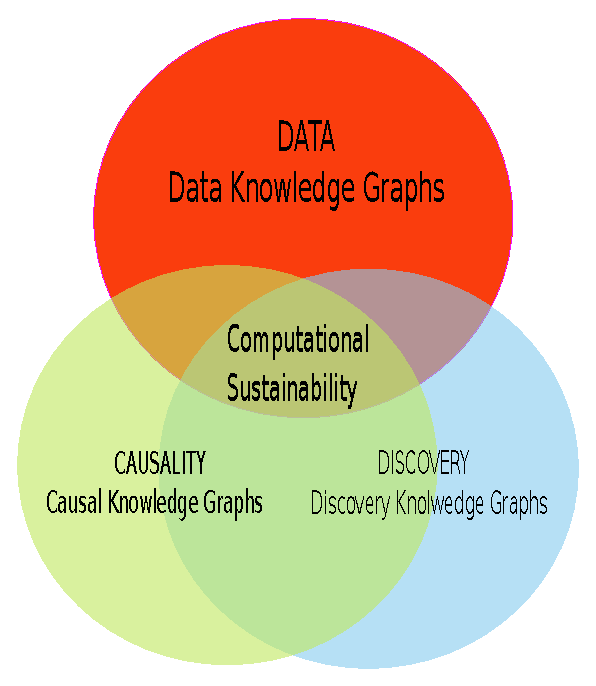
\includegraphics[width = 0.5\textwidth]{Fig0.pdf}\\
	 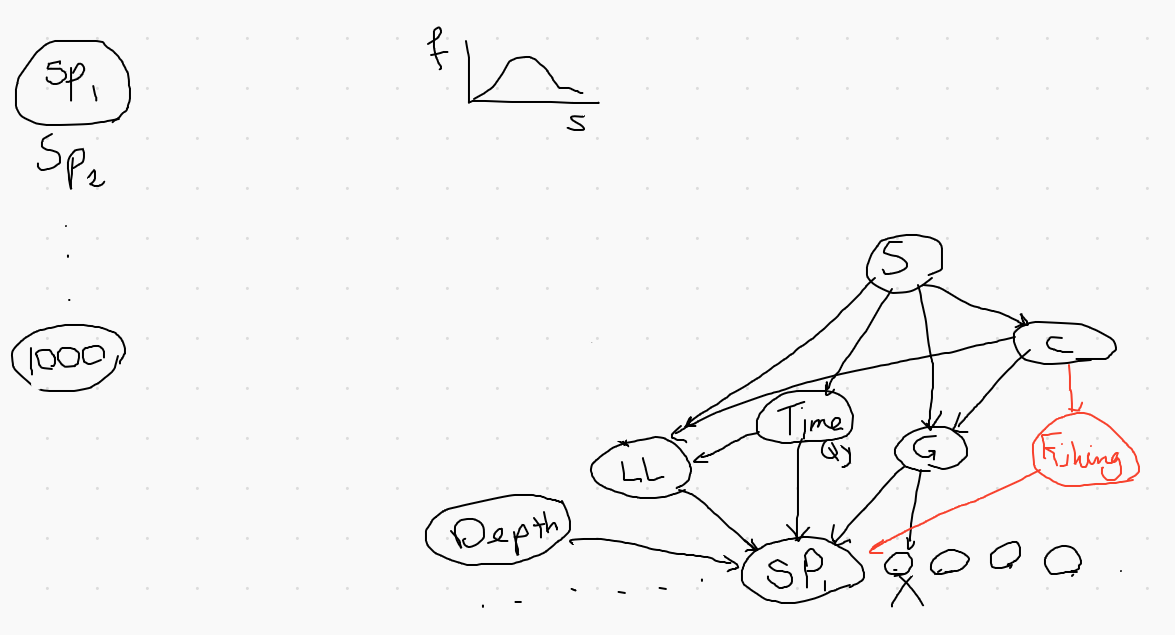
\includegraphics[width = 1\textwidth]{Fig1BN.png}
	 \caption{Computational sustainability is at the intersection of data, causality and discovery knowledge graphs. Data knowledge graphs introduces data fussion and semantics to disparate database. Causality knowledge graphs makes inferences about the processes explaining the empirical patterns observed in the data knowledge graphs. Discovery knowledge graphs finds novel paths not observed in the empirical patterns but of relevance to increase sustainability.}
\end{figure}   

\begin{figure}[H]
	 \centering
	 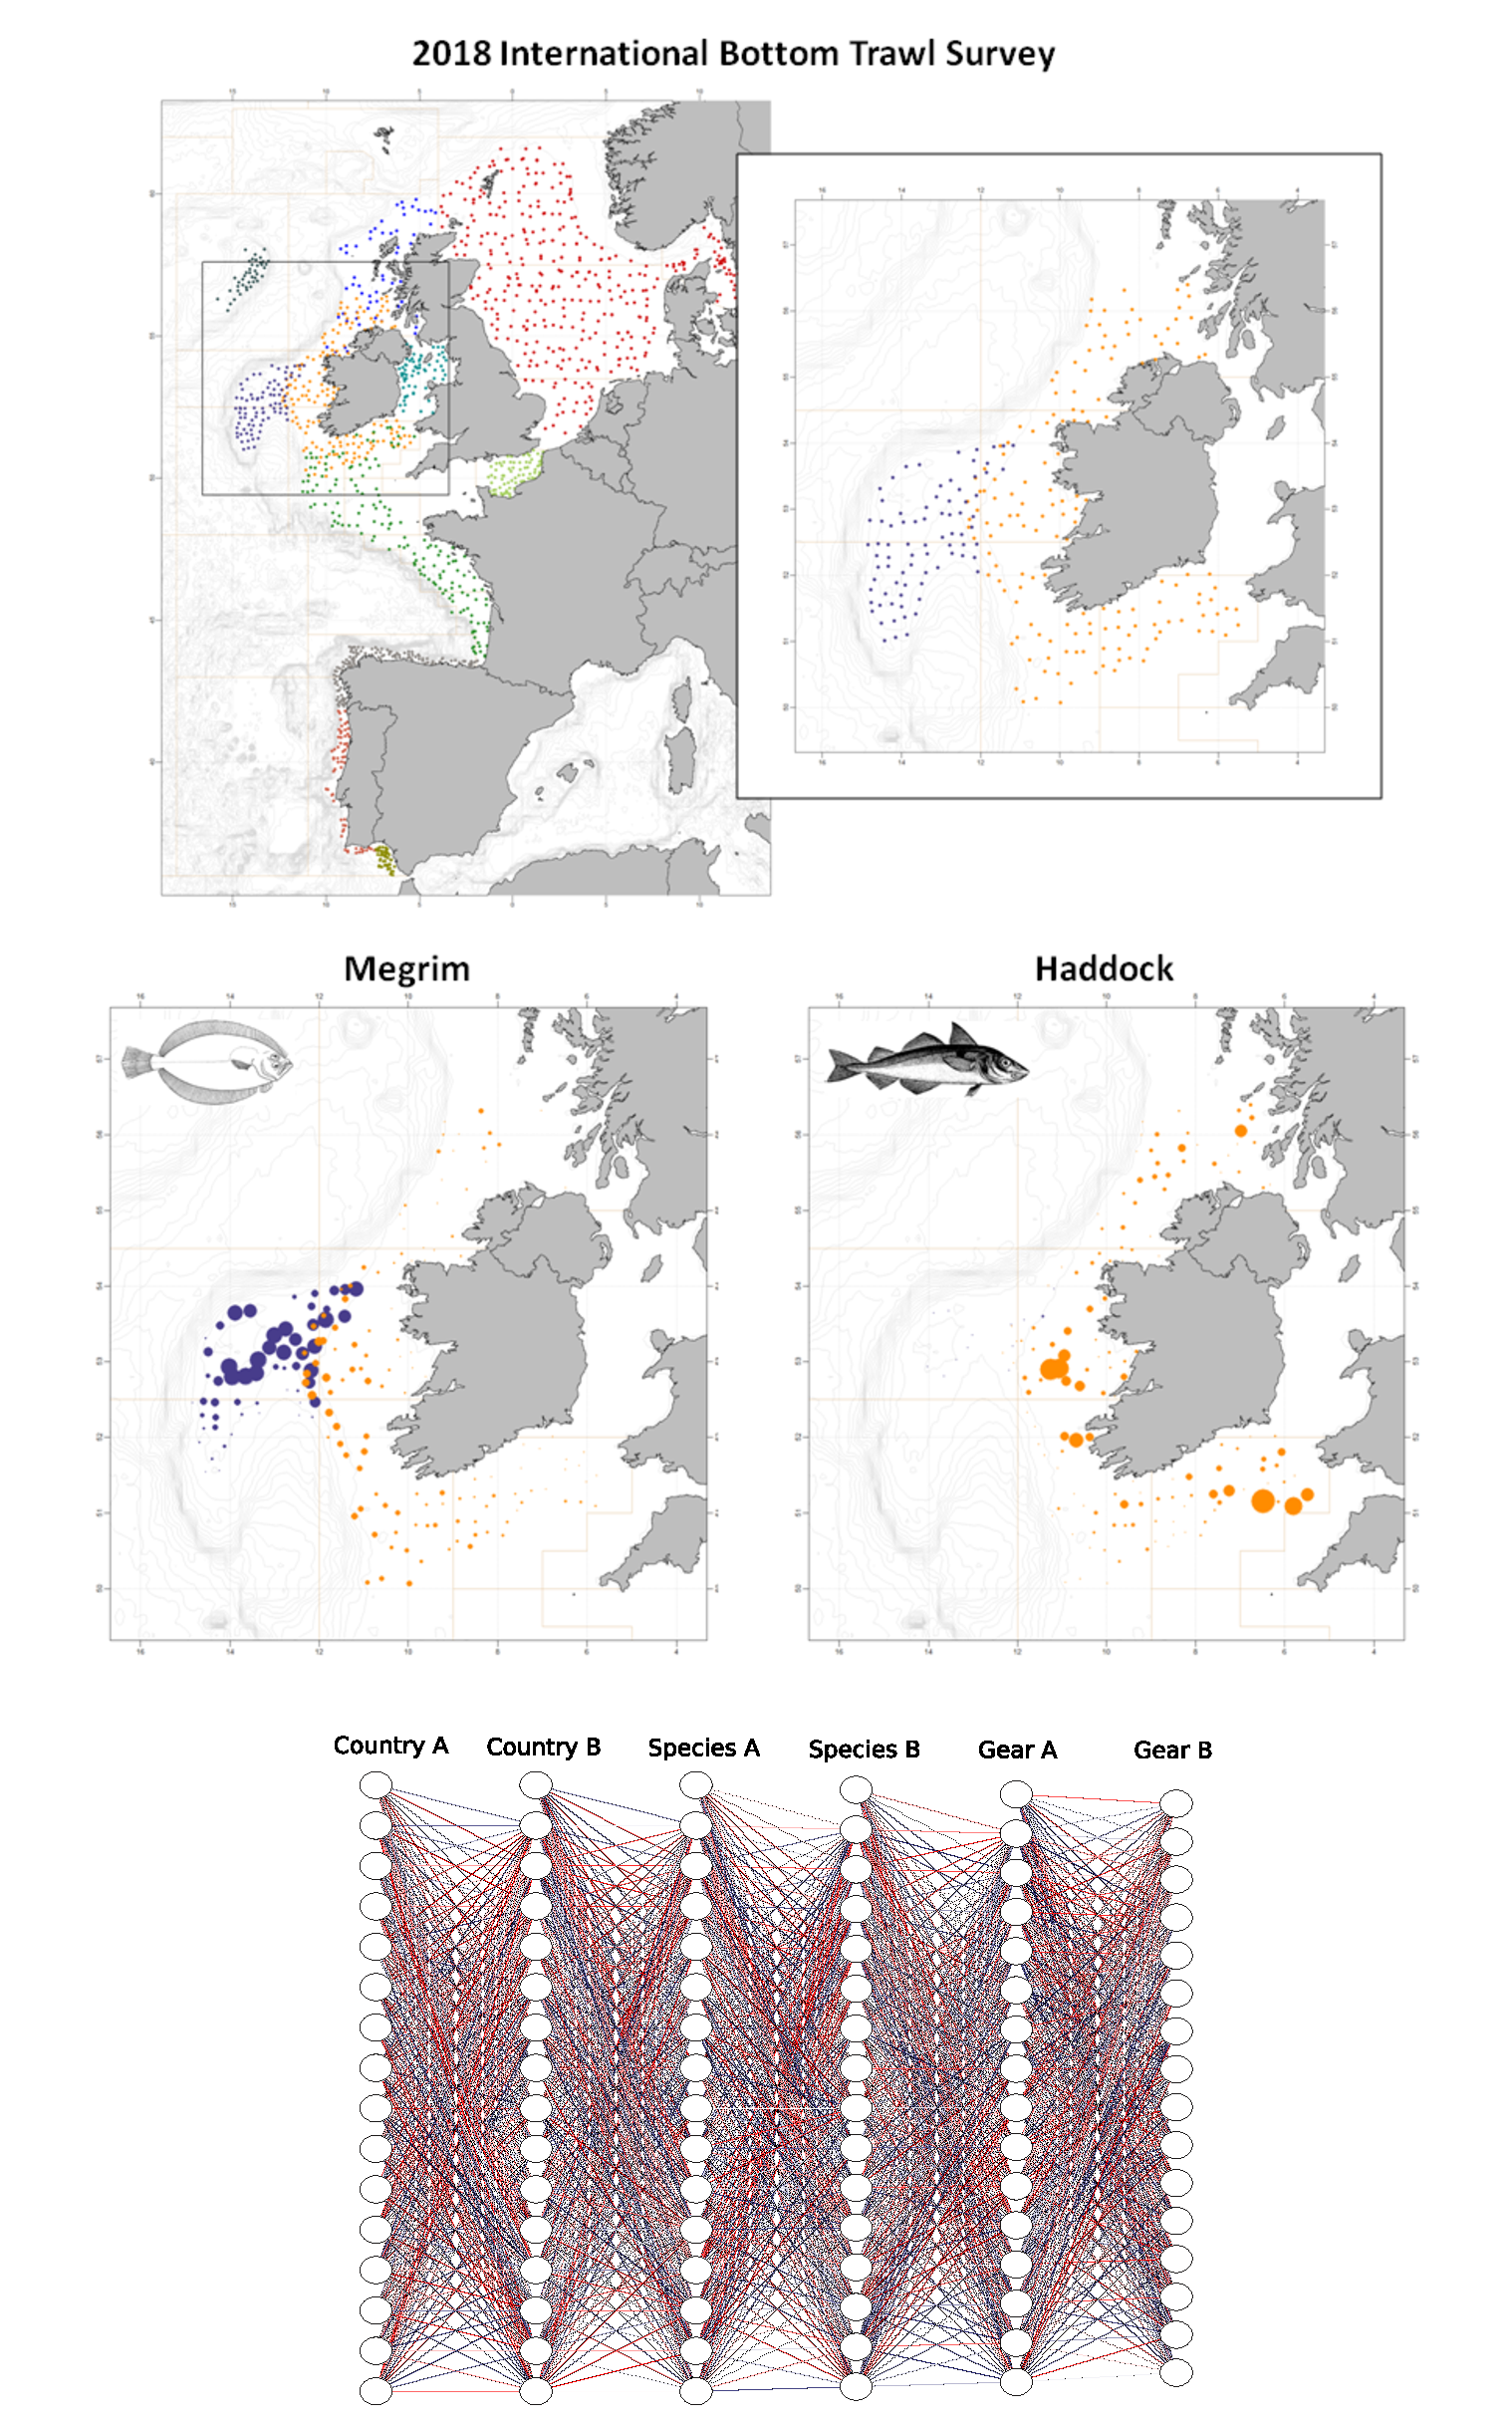
\includegraphics[width = 0.75\textwidth]{casestudy.pdf}
	 \caption{Computational sustainability applied to the sustainability of the Oceans case study combining many species, human groups and technologies. Top left) Zoomed in is the Irish Ground Fish Survey (IE-IGFS, Orange) and the Spanish Survey on the Porcupine Bank (PORC, Blue). Countries produce strong bias in the distributions maps because they use different Gears according to their commercial interest (Compare Megrim vs. Haddock samplings). Bottom) Each country, species and technology composed of many nodes: country contains fishery, environmental agencies, stakeholders, etc. Species contains size-classes, habitat preference, species interactions, etc. Red and blue links mean competition and cooperation links connecting each pair of nodes.}
\end{figure}

\begin{figure}[H]
	 \centering
	 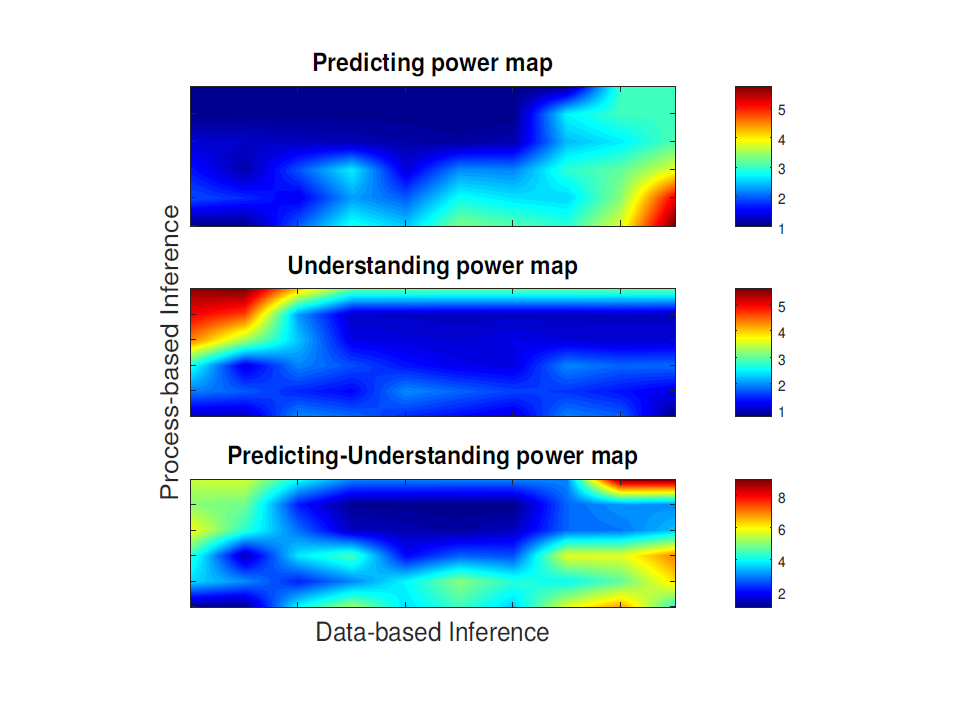
\includegraphics[width = 1\textwidth]{Fig1.png}
	 \\
	 \caption{CAPTION TO BE INCLUDED}
      \end{figure}

\begin{figure}[H]
	\centering
	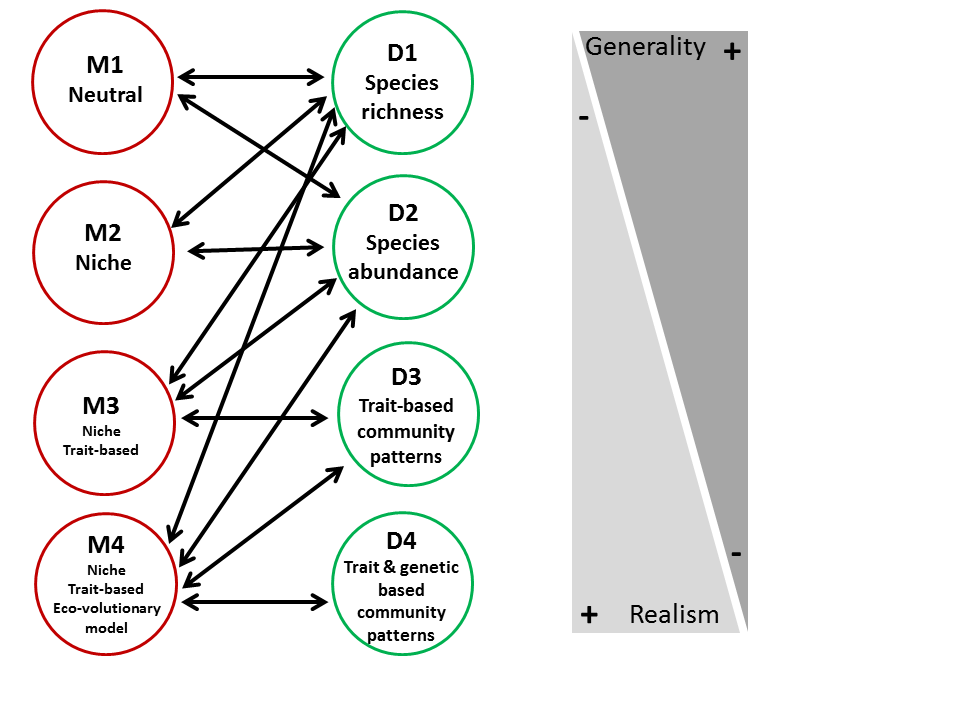
\includegraphics[width = 1\textwidth]{Fig2.png}
	\caption{Integration between models (M1-M4) and datasets (D1-D4). As model complexity increases (i.e., Realism) models produce more number of testable outputs but generality and tractability might decrease}
\end{figure}


\newpage
\bibliographystyle{evolution}
\bibliography{Biblio_deepbios}

\end{document}
